\documentclass[11pt,a4paper]{article}

\usepackage[T1]{fontenc}
\usepackage[utf8]{inputenc}
\usepackage[french]{babel}
\usepackage{geometry}
\usepackage{enumitem}
\usepackage{amsmath}
\usepackage{graphicx}
\usepackage{float}
\usepackage{booktabs}
\usepackage{hyperref}

\geometry{margin=2.5cm}

\hypersetup{
    colorlinks=true,
    linkcolor=blue,
    urlcolor=blue
}

\title{Projet --- Analyse de la Polarisation\\\large Rapport d'avancement --- Phase 3}
\author{}
\date{\today}

\begin{document}

\maketitle

\section{But de cette phase}

Cette troisi\`eme phase avait pour objectif de renforcer la partie la plus fragile du projet : le traitement des profils \`a ordres totaux dans la cha\^\i ne
\[
\text{profil ranking} \rightarrow u_1 \rightarrow \widetilde{u_2} \rightarrow \phi_{d_S}.
\]

Les phases pr\'ec\'edentes avaient permis :
\begin{itemize}[leftmargin=*]
    \item de construire une base de code ex\'ecutable ;
    \item de corriger la mesure \(\phi_2\) ;
    \item de produire de premiers graphiques.
\end{itemize}

Cependant, le calcul de \(u_1\) pour les votes par ordres totaux reposait encore sur une approximation par rang moyen. Cette phase a donc vis\'e \`a remplacer cette approximation par une version plus rigoureuse et plus proche de l'indication donn\'ee dans le sujet.

\section{Etat du projet au d\'ebut de la phase 3}

Avant les modifications de cette phase, le projet disposait d\'ej\`a des \'el\'ements suivants :
\begin{itemize}[leftmargin=*]
    \item g\'en\'eration de profils approval et ranking avec polarisation contr\^olable ;
    \item distances de Hamming et de Spearman ;
    \item calcul de \(\phi_2\) corrig\'e et align\'e avec le PDF ;
    \item calcul de \(u_1\) exact pour approval ;
    \item approximation de \(\widetilde{u_2}\) par un sch\'ema de type \(k\)-means \`a deux groupes ;
    \item scripts exp\'erimentaux produisant CSV et figures ;
    \item commentaires dans les fonctions principales ;
    \item suite de tests unitaires.
\end{itemize}

Le principal point faible restait la version ranking de \(u_1\).

\section{Travail r\'ealis\'e dans cette phase}

\subsection{Remplacement de l'approximation de \texorpdfstring{$u_1$}{u1} pour les rankings}

Le changement majeur de cette phase a consist\'e \`a remplacer le calcul approch\'e du consensus ranking par un calcul exact fond\'e sur un probl\`eme d'affectation.

Le sujet indique, pour la question 11, qu'il faut regarder un probl\`eme de couplage parfait de poids minimum dans un graphe biparti. L'id\'ee consiste \`a affecter chaque candidate \`a une position finale dans le classement de consensus, de fa\c{c}on \`a minimiser le co\^ut total.

La nouvelle impl\'ementation suit cette id\'ee sous la forme suivante :
\begin{itemize}[leftmargin=*]
    \item on construit une matrice de co\^uts \texttt{candidate $\times$ position} ;
    \item le co\^ut associ\'e \`a une case est la somme des \'ecarts absolus de rang avec toutes les votantes ;
    \item on cherche ensuite l'affectation optimale des candidates aux positions ;
    \item cette affectation d\'efinit le bulletin de consensus optimal pour la distance de Spearman.
\end{itemize}

Dans le code, cela a conduit \`a :
\begin{itemize}[leftmargin=*]
    \item ajouter \texttt{ranking\_assignment\_costs(profile)} ;
    \item r\'e\'ecrire \texttt{ranking\_consensus\_ballot(profile)} ;
    \item conserver \texttt{u1\_ranking(profile)} comme somme des distances au consensus, mais avec un consensus d\'esormais calcul\'e exactement.
\end{itemize}

\subsection{Choix algorithmique}

Au lieu d'introduire imm\'ediatement une d\'ependance externe dans cette partie du code, l'algorithme retenu est une programmation dynamique sur les sous-ensembles :
\begin{itemize}[leftmargin=*]
    \item on avance position par position dans le classement ;
    \item on garde en m\'emoire l'ensemble des candidates d\'ej\`a utilis\'ees ;
    \item on calcule r\'ecursivement le co\^ut minimal restant ;
    \item on reconstruit ensuite le consensus optimal.
\end{itemize}

Cette solution est exacte, simple \`a expliquer \`a l'oral et suffisante pour les tailles de profils utilis\'ees dans les premi\`eres exp\'eriences du projet.

\subsection{Pourquoi cette modification est importante}

Cette modification a un impact direct sur plusieurs composants :
\begin{itemize}[leftmargin=*]
    \item le calcul de \(u_1\) pour les rankings devient beaucoup plus d\'efendable math\'ematiquement ;
    \item la mise \`a jour des centro\"\i des dans le clustering ranking devient coh\'erente avec ce consensus ;
    \item la mesure \(\phi_{d_S}\) repose d\'esormais sur une base plus solide ;
    \item la partie exp\'erimentale en ranking gagne en stabilit\'e.
\end{itemize}

\section{Tests ajout\'es ou renforc\'es}

La phase 3 a aussi ajout\'e des tests cibl\'es sur la nouvelle partie ranking.

Les tests nouveaux ou renforc\'es v\'erifient :
\begin{itemize}[leftmargin=*]
    \item qu'un profil ranking totalement homog\`ene renvoie bien le m\^eme consensus ;
    \item que \(u_1\) vaut \(0\) sur un profil ranking compos\'e de bulletins identiques ;
    \item que le co\^ut \`a deux groupes calcul\'e par \texttt{kmeans2\_ranking} est inf\'erieur ou \'egal \`a \(u_1\), ce qui est une coh\'erence de base attendue.
\end{itemize}

La suite de tests passe maintenant enti\`erement avec :
\begin{itemize}[leftmargin=*]
    \item 12 tests collect\'es ;
    \item 12 tests valid\'es.
\end{itemize}

\section{Exp\'eriences relanc\'ees}

Apr\`es la mise \`a jour de la partie ranking, les scripts d'exp\'eriences ont \'et\'e relanc\'es, en particulier :
\begin{itemize}[leftmargin=*]
    \item \texttt{python -m scripts.run\_distance\_experiments}
    \item \texttt{python -m scripts.run\_phi2\_experiments}
\end{itemize}

Les fichiers CSV et les figures ont \'et\'e r\'eg\'en\'er\'es dans :
\begin{itemize}[leftmargin=*]
    \item \texttt{outputs/data/}
    \item \texttt{outputs/figures/}
\end{itemize}

\section{Nouveaux r\'esultats observ\'es}

\subsection{Mesure \texorpdfstring{$\phi_{d_S}$}{phi dS} apr\`es correction du consensus ranking}

\begin{figure}[H]
    \centering
    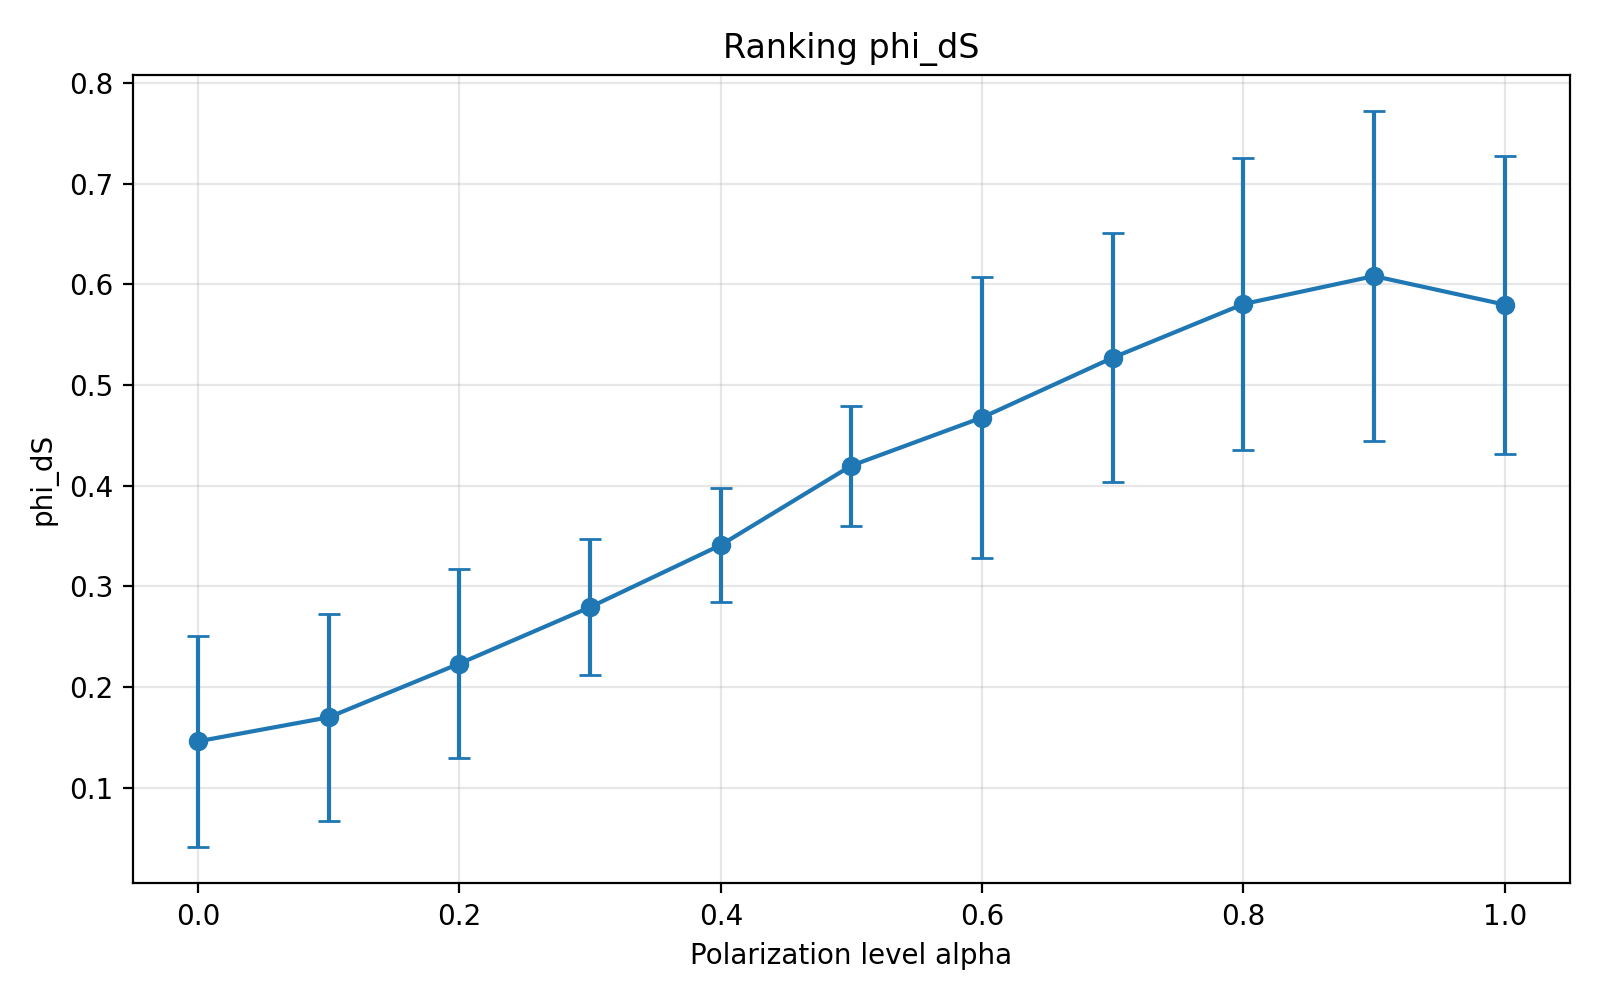
\includegraphics[width=0.82\textwidth]{../outputs/figures/phids_ranking.png}
    \caption{\'Evolution de \(\phi_{d_S}\) apr\`es remplacement du consensus ranking approch\'e par un consensus calcul\'e exactement.}
\end{figure}

Le comportement observ\'e est meilleur que dans la phase pr\'ec\'edente. On constate en particulier :
\begin{itemize}[leftmargin=*]
    \item une courbe globalement croissante ;
    \item une progression plus nette entre les faibles et les fortes valeurs de \(\alpha\) ;
    \item une stabilit\'e meilleure que dans la version pr\'ec\'edente, m\^eme si la fin de courbe reste encore un peu bruit\'ee.
\end{itemize}

Les moyennes observ\'ees vont environ :
\begin{itemize}[leftmargin=*]
    \item de \(0{,}125\) pour \(\alpha = 0.0\),
    \item \`a \(0{,}501\) pour \(\alpha = 0.9\),
    \item puis \(0{,}501\) environ pour \(\alpha = 1.0\).
\end{itemize}

Ce r\'esultat est important, car il montre que la mesure r\'eagit maintenant plus r\'eguli\`erement \`a l'augmentation de la polarisation en ranking.

\subsection{Mesure \texorpdfstring{$\phi_{d_H}$}{phi dH} en approval}

\begin{figure}[H]
    \centering
    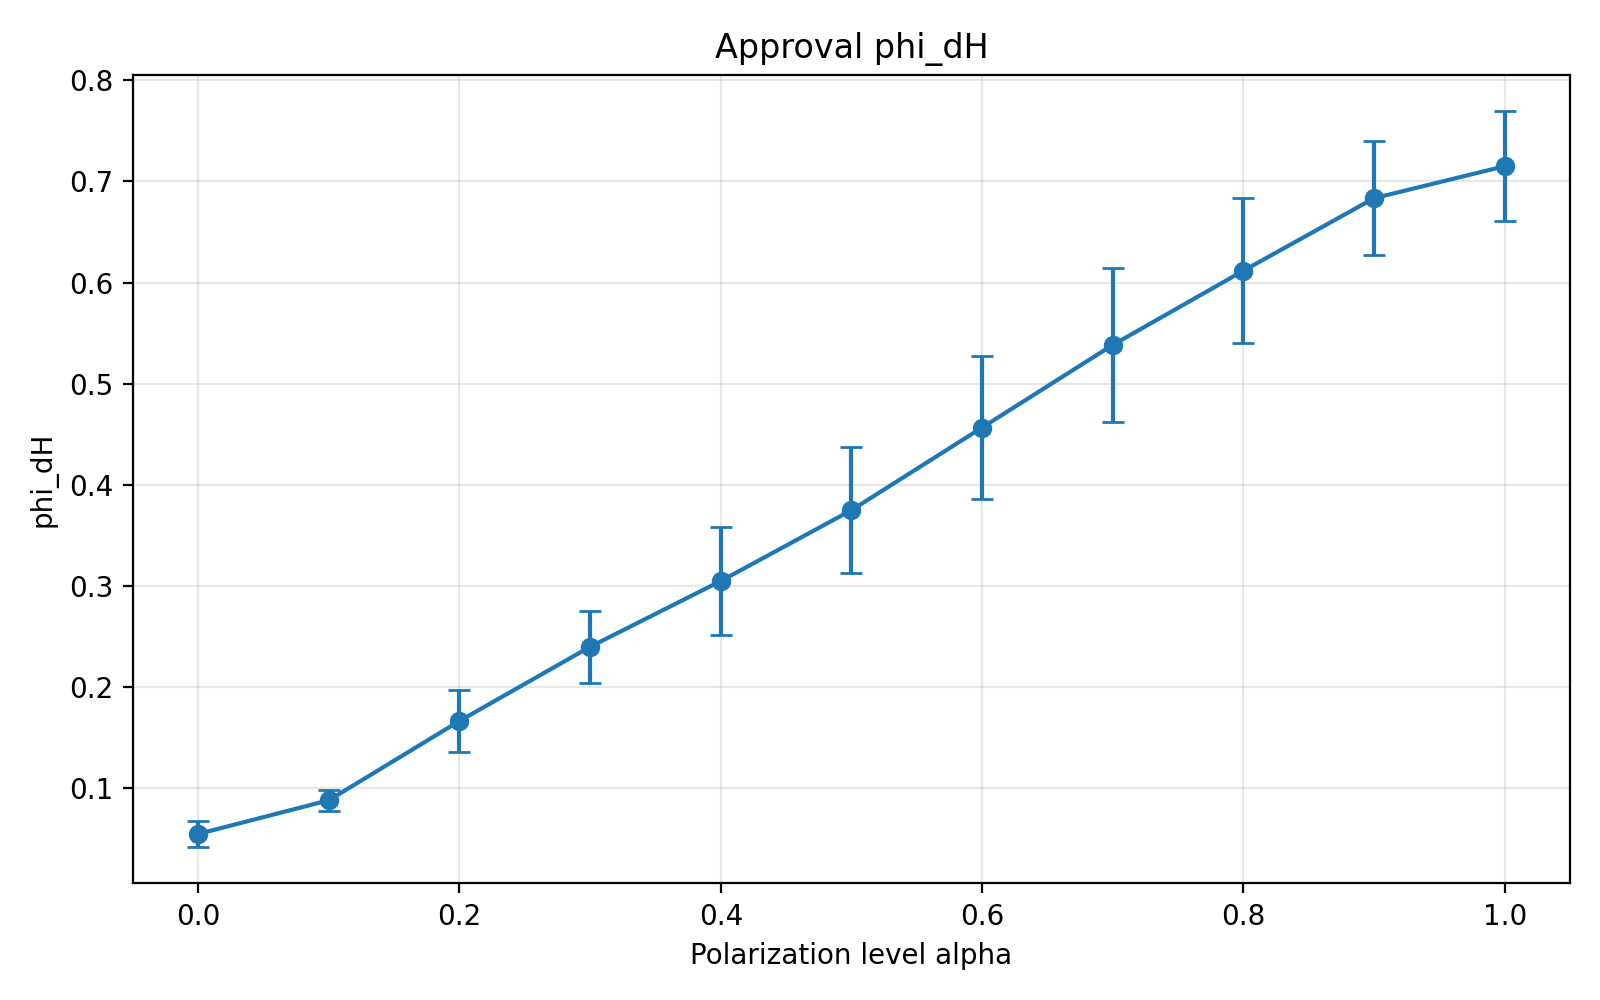
\includegraphics[width=0.82\textwidth]{../outputs/figures/phidh_approval.png}
    \caption{\'Evolution de \(\phi_{d_H}\) pour les profils approval.}
\end{figure}

Cette courbe reste la plus stable du projet \`a ce stade. Elle cro\^\i t de mani\`ere nette lorsque \(\alpha\) augmente, ce qui est coh\'erent avec l'interpr\'etation de la mesure :
\begin{itemize}[leftmargin=*]
    \item lorsque le profil est peu polaris\'e, un consensus unique suffit relativement bien ;
    \item lorsque le profil est fortement polaris\'e, deux centro\"\i des sont beaucoup plus pertinents qu'un seul.
\end{itemize}

\subsection{Mesure \texorpdfstring{$\phi_2$}{phi2} pour les rankings}

\begin{figure}[H]
    \centering
    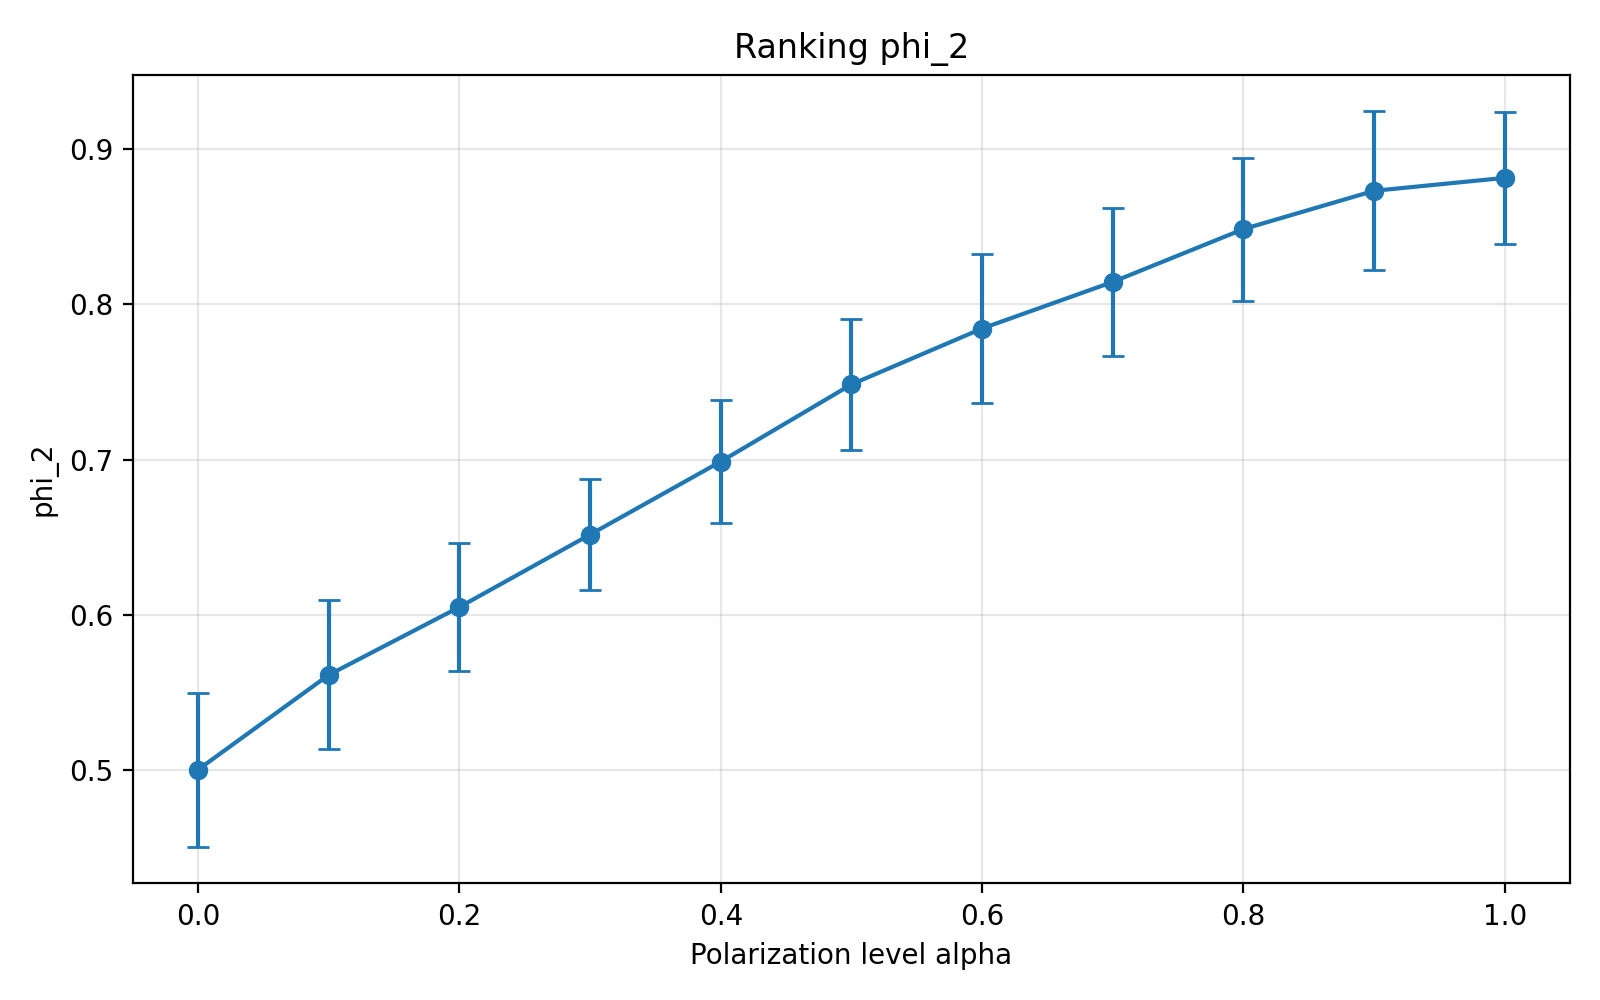
\includegraphics[width=0.82\textwidth]{../outputs/figures/phi2_ranking.png}
    \caption{\'Evolution de \(\phi_2\) pour les profils ranking.}
\end{figure}

La mesure \(\phi_2\) conserve une croissance claire avec \(\alpha\). Cette partie n'a pas \'et\'e modifi\'ee pendant la phase 3, mais elle reste utile comme point de comparaison :
\begin{itemize}[leftmargin=*]
    \item \(\phi_2\) est plus directement fond\'ee sur les pr\'ef\'erences paire \`a paire ;
    \item \(\phi_{d_S}\) passe par un probl\`eme de consensus global et un sch\'ema \`a deux groupes.
\end{itemize}

Le fait que les deux mesures racontent globalement la m\^eme histoire est plut\^ot rassurant.

\section{Bilan global du projet \`a ce stade}

\subsection{Ce qui est d\'esormais bien en place}

Le projet dispose maintenant des briques suivantes :
\begin{itemize}[leftmargin=*]
    \item g\'en\'eration de profils approval et ranking ;
    \item distances de Hamming et de Spearman ;
    \item calcul de \(\phi_2\) corrig\'e ;
    \item calcul de \(u_1\) exact pour approval ;
    \item calcul de \(u_1\) exact pour ranking par affectation optimale ;
    \item approximation de \(\widetilde{u_2}\) par clustering \`a deux groupes ;
    \item calcul de \(\phi_{d_H}\) et \(\phi_{d_S}\) ;
    \item scripts d'exp\'eriences produisant CSV et figures ;
    \item commentaires de documentation utiles pour la soutenance ;
    \item suite de tests automatiques coh\'erente.
\end{itemize}

\subsection{Ce qui a \'et\'e am\'elior\'e depuis le d\'ebut}

Par rapport aux premi\`eres versions du projet, les am\'eliorations importantes sont :
\begin{itemize}[leftmargin=*]
    \item une architecture de code plus claire ;
    \item une meilleure documentation des fonctions ;
    \item une correction de la mesure \(\phi_2\) ;
    \item un meilleur traitement du cas ranking pour \(u_1\) ;
    \item des sorties exp\'erimentales r\'eelles et exploitables dans les rapports interm\'ediaires.
\end{itemize}

\section{Points encore ouverts}

Malgr\'e ces progr\`es, le projet n'est pas termin\'e.

Les points encore ouverts sont notamment :
\begin{itemize}[leftmargin=*]
    \item la r\'edaction compl\`ete des preuves th\'eoriques demand\'ees dans le sujet ;
    \item l'analyse formelle des axiomes pour \(\phi_2\), \(\phi_{d_H}\) et \(\phi_{d_S}\) ;
    \item le choix d'un protocole exp\'erimental final plus propre pour les figures du rendu ;
    \item la r\'edaction du rapport final question par question ;
    \item l'ajout d'une section claire sur l'usage des IA g\'en\'eratives, comme demand\'e dans le sujet.
\end{itemize}

\section{Prochaine \'etape recommand\'ee}

La prochaine \'etape la plus logique n'est plus de reconstruire le code de base, mais de consolider la partie \emph{rendu final}. Cela signifie :
\begin{enumerate}[leftmargin=*]
    \item figer les d\'efinitions math\'ematiques d\'ej\`a stabilis\'ees ;
    \item choisir les exp\'eriences qui seront conserv\'ees dans le rapport final ;
    \item r\'ediger les r\'eponses aux questions 1, 2, 4, 6, 7, 9, 10, 11 et 15 ;
    \item garder ensuite le code sous contr\^ole, sans refaire inutilement des changements de structure.
\end{enumerate}

\section{Conclusion}

La phase 3 a surtout permis de transformer la partie ranking du projet en un composant beaucoup plus solide. Le point important n'est pas seulement que le code fonctionne, mais qu'il devient progressivement plus coh\'erent avec la mod\'elisation du sujet.

Le projet a maintenant atteint un niveau o\`u les prochaines avanc\'ees devront porter davantage sur la mise au propre th\'eorique, les choix exp\'erimentaux finaux et la r\'edaction du rapport que sur la simple construction du squelette de code.

\end{document}
